% Load the kaobook class
\documentclass[
	fontsize=10pt, % Base font size
	twoside=false, % Use different layouts for even and odd pages (in particular, if twoside=true, the margin column will be always on the outside)
	%open=any, % If twoside=true, uncomment this to force new chapters to start on any page, not only on right (odd) pages
	secnumdepth=1, % How deep to number headings. Defaults to 1 (sections)
]{kaobook}

% Choose the language
\usepackage[english]{babel} % Load characters and hyphenation
\usepackage[english=british]{csquotes}	% English quotes

% === CUSTOM THINGS ===
\usepackage{mycommands}

% Load the bibliography package
\usepackage[style=numeric,sorting=none]{kaobiblio}  
% \usepackage[style=numeric,sorting=none]{biblatex}
\addbibresource{./BA.bib}

\usepackage{subcaption}

% ======

% Load packages for testing
\usepackage{blindtext}
%\usepackage{showframe} % Uncomment to show boxes around the text area, margin, header and footer
%\usepackage{showlabels} % Uncomment to output the content of \label commands to the document where they are used
  

% Load mathematical packages for theorems and related environments
\usepackage{kaotheorems}

% Load the package for hyperreferences
\usepackage{kaorefs}

\graphicspath{{images/}{./}} % Paths where images are looked for

\makeindex[columns=3, title=Alphabetical Index, intoc] % Make LaTeX produce the files required to compile the index


\begin{document}

%----------------------------------------------------------------------------------------
%	BOOK INFORMATION
%----------------------------------------------------------------------------------------

% \titlehead{Document Template}
\title[Node Duplication in Disease Maps using Graph Neural Networks]{Node
  Duplication in Disease Maps using Graph Neural Networks}
\author[BM]{Benjamin Moser}
\date{\today}
% \publishers{An Awesome Publisher}

%----------------------------------------------------------------------------------------

\frontmatter % Denotes the start of the pre-document content, uses roman numerals

%----------------------------------------------------------------------------------------
%	COPYRIGHT PAGE
%----------------------------------------------------------------------------------------

\makeatletter
\uppertitleback{\@titlehead} % Header

\lowertitleback{
	\textbf{Disclaimer} \\
	You can edit this page to suit your needs. For instance, here we have a no copyright statement, a colophon and some other information. This page is based on the corresponding page of Ken Arroyo Ohori's thesis, with minimal changes.
	
	\medskip
	
	\textbf{No copyright} \\
	\cczero\ This book is released into the public domain using the CC0 code. To the extent possible under law, I waive all copyright and related or neighbouring rights to this work.
	
	To view a copy of the CC0 code, visit: \\\url{http://creativecommons.org/publicdomain/zero/1.0/}
	
	\medskip
	
	\textbf{Colophon} \\
	This document was typeset with the help of \href{https://sourceforge.net/projects/koma-script/}{\KOMAScript} and \href{https://www.latex-project.org/}{\LaTeX} using the \href{https://github.com/fmarotta/kaobook/}{kaobook} class.
	
	\medskip
	
	\textbf{Publisher} \\
	First printed in May 2019 by \@publishers
}
\makeatother

%----------------------------------------------------------------------------------------
%	DEDICATION
%----------------------------------------------------------------------------------------

\dedication{
	The harmony of the world is made manifest in Form and Number, and the heart and soul and all the poetry of Natural Philosophy are embodied in the concept of mathematical beauty.\\
	\flushright -- D'Arcy Wentworth Thompson
}

%----------------------------------------------------------------------------------------
%	OUTPUT TITLE PAGE AND PREVIOUS
%----------------------------------------------------------------------------------------

% Note that \maketitle outputs the pages before here
\maketitle

%----------------------------------------------------------------------------------------
%	PREFACE
%----------------------------------------------------------------------------------------

\chapter*{Preface}

\blindtext

%----------------------------------------------------------------------------------------
%	TABLE OF CONTENTS & LIST OF FIGURES/TABLES
%----------------------------------------------------------------------------------------

\begingroup % Local scope for the following commands

% Define the style for the TOC, LOF, and LOT
%\setstretch{1} % Uncomment to modify line spacing in the ToC
%\hypersetup{linkcolor=blue} % Uncomment to set the colour of links in the ToC
\setlength{\textheight}{230\vscale} % Manually adjust the height of the ToC pages

% Turn on compatibility mode for the etoc package
\etocstandarddisplaystyle % "toc display" as if etoc was not loaded
\etocstandardlines % "toc lines as if etoc was not loaded

\tableofcontents % Output the table of contents

\listoffigures % Output the list of figures

% Comment both of the following lines to have the LOF and the LOT on different pages
\let\cleardoublepage\bigskip
\let\clearpage\bigskip

\listoftables % Output the list of tables

\section{Notation}
% TODO bipartite graph
% TODO bipartite projection / clique reduction

\endgroup

%----------------------------------------------------------------------------------------
%	MAIN BODY
%----------------------------------------------------------------------------------------

\mainmatter % Denotes the start of the main document content, resets page numbering and uses arabic numbers
\setchapterstyle{plain} % Choose the default chapter heading style

\pagelayout{wide} % No margins

\chapter{Introduction}
\blindtext

\section{Biological Networks}
Our understanding of the molecular mechanisms that are involved in biological
systems is improving drastically. However, this knowledge is growing
incrementally and is often scattered across individual scientific publications.
The behaviour of a biological system is often defined by complex interactions,
potentially across different levels of abstraction. We refer to biological
entities as \textit{species}. Possible species types are, for instance,
proteins, genes, but possibly also abstract phenotype descriptions or drugs.
%
Possible relations include chemical reactions such as state transition (e.g.
phosphorylation), physical interaction between two proteins or the effect a drug
has on the function of some protein.
%
The set of species and their interactions (relationships) naturally form a
network. To properly consider complex signalling effects such as
activation/inhibition, crosstalk or feedback, it is of the essence to make this
network structure accessible to both human cognition and computational analysis
\cite{barabasi_NetworkBiologyUnderstanding_2004}.

Choices of what species and relationships to consider yield different flavours
of biological networks and analyses. Since the effective biological function of
proteins is rarely defined solely by their identity but rather by their roles as
enzymes, signalling molecules or structural components, it is worthwhile to
study \ild{Protein-Protein Interaction Networks} (\textsc{PPI} networks), for
instance to infer the biological function of an unknown protein or gene, or
groups of functionally similar proteins.
% TODO more cites
Further, an organism's metabolism may
be described as a set of chemical compounds (metabolites) and the set of
chemical reactions or interactions between them, yielding a \ild{metabolic
  model}. Computational methods on metabolic networks can be used to predict the
growth of an organism under specific conditions, identify key intervention
targets or decompose the network into relatively independent subsystems.
% TODO citations
However, species and relationships need not necessarily have a direct physical
counterpart. Several works investigate the interactions between diseases, drugs,
proteins and their annotated biological functions
\cite{ruiz_identification_2021} \cite{barabasi_NetworkMedicineNetworkbased_2011}.
% TODO cite that work on gene classification for cancer thing presented by janina
% TODO cite more
Moreover, biological networks may serve as a scaffold to integrate data on,
e.g., gene expression or reaction rates. This can be used to classify cancer
% TODO more precise and cite, the work I looked at for prop for whole-graph
% classification
or TODO.

\section{Disease Maps}

Biochemical pathways can be described by \ild{process description diagrams} in
which species (commonly metabolites, protein complexes and genes) are linked by
chemical processes. An example is given in \reffig{fig:process-diagram-old-vs-new}.
%
Many diseases, however, affect not only a single mechanism. Rather, a systemic
understanding of the involved subsystem and their relationships is required
\cite{ostaszewski_CommunitydrivenRoadmapIntegrated_2019}\cite{mazein_SystemsMedicineDisease_2018}.
%
Moreover, knowledge on mechanisms contributing to a disease is obtained
incrementally and scattered across individual publications or database entries.
%
Particularly for visual, interactive exploration, experts have assembled
\ild{disease maps}, comprehensive diagrams combining all known mechanisms
relevant for a given disease.
%
Traditionally, such diagrams have been drawn as pixel- or vector-based graphics.
Creating and updating such graphics requries a high amount of effort and renders
the contained information practically inaccessible to computational methods.
%
Formalised, digital representations that are both human- and computer-readable
provide the following immediate advantages. 
\begin{itemize}
\item The creation process, involving the extraction of knowledge from
  scientific publications or databases and finding an adequate layout, may be
  aided by computational tools from the areas of Data Mining and Graph Drawing.
  \item Entities in the diagram may be annotated with additional information
    such as links to research publication or database entries.
\item A formalised representation enables the use of computational methods for
  analysis and interactive exploration (see \nameref{sec:related-work} for examples).
\item Diagrams provide a formalized model that can serve as a scaffold for
  integrating \textit{multi-omics} data. % TODO more
\end{itemize}

Although their content is based on biological processes, disease maps differ in
nature from other types of biological networks in the following aspects:
\begin{itemize}
\item The contents of a disease map are assembled based on the judgement of one
  or several curators. Only processes that are deemed relevant or informative to
  the given objective are included.
\item A disease map is an actual visual diagram, i.e. visual representations of
  species and relationships have been laid out to optimally present the included
  information. Although several approaches for the drawing of large process
  diagrams exist (see TODO), it is still common practise
  to invest manual effort into the layout.
\end{itemize}
The above points also show that such maps are inherently subjective.

Recent disease maps contain up to several thousands of species and reactions and
are very rich in information beyond the mere enumeration of species and their
pairwise relationships. To give only a few examples: different types of species
and relationships (as described above) are explicitly encoded. Further, species
can be assigned relative positions to a biological compartment they reside in.
Species can be assigned different states (e.g. ``phosphorylated'') and form
\textit{complexes} (groups). Further, species and relationships are often
annotated with links to external databases such as Entrez Gene
\cite{maglott_EntrezGeneGenecentered_2005} or UniProt
\cite{theuniprotconsortium_UniProtUniversalProtein_2021}.

% TODO (low) how are disease maps created?

% TODO update nameref s.t. name is put in quotation marks

To date, disease maps have been created for a number of diseases, including Alzheimer's
Disease (\alzpathway \cite{ogishima_AlzPathwayUpdatedMap_2016}), Parkinson's Disease
(\pdmap \cite{fujita_IntegratingPathwaysParkinson_2014}), and recently \textsc{COVID-19}
\cite{ostaszewski_COVID19DiseaseMap_2020}. Beyond serving as a platform for
integrating existing knowledge, computational methods have been applied to,
e.g., identify molecules and relations essential for the pathogenesis of Alzheimer's
Disease \cite{mizuno_NetworkAnalysisComprehensive_2016}. Detailed information on
the disease maps considered in this work can be found in \refsec{sec:datasets}.

Several tools exist for the curation and exploration of such diagrams, including
\toolname{CellDesigner} \cite{funahashi_CellDesignerVersatileModeling_2008},
\toolname{Minerva} \cite{gawron_MINERVAPlatformVisualization_2016}, and
\toolname{Cytoscape} \cite{shannon_cytoscape_2003} and \toolname{VANTED}
\cite{rohn_VANTEDV2Framework_2012}. We refer to TODO for a comprehensive
comparison.
% TODO use \toolname in this paragraph
One of the most common formats used for describing disease maps is an extension to SBML
Level 2 given by \toolname{CellDesigner}. Further, SBML Level 3 now allows to attach
layout information. Another prominent format is SBGN-ML.
% TODO footnote for abbreviations
% TODO citations for SBML, SBGN-ML

\begin{figure}[b]
  \centering
  \begin{subfigure}{0.4\textwidth}
    \centering
    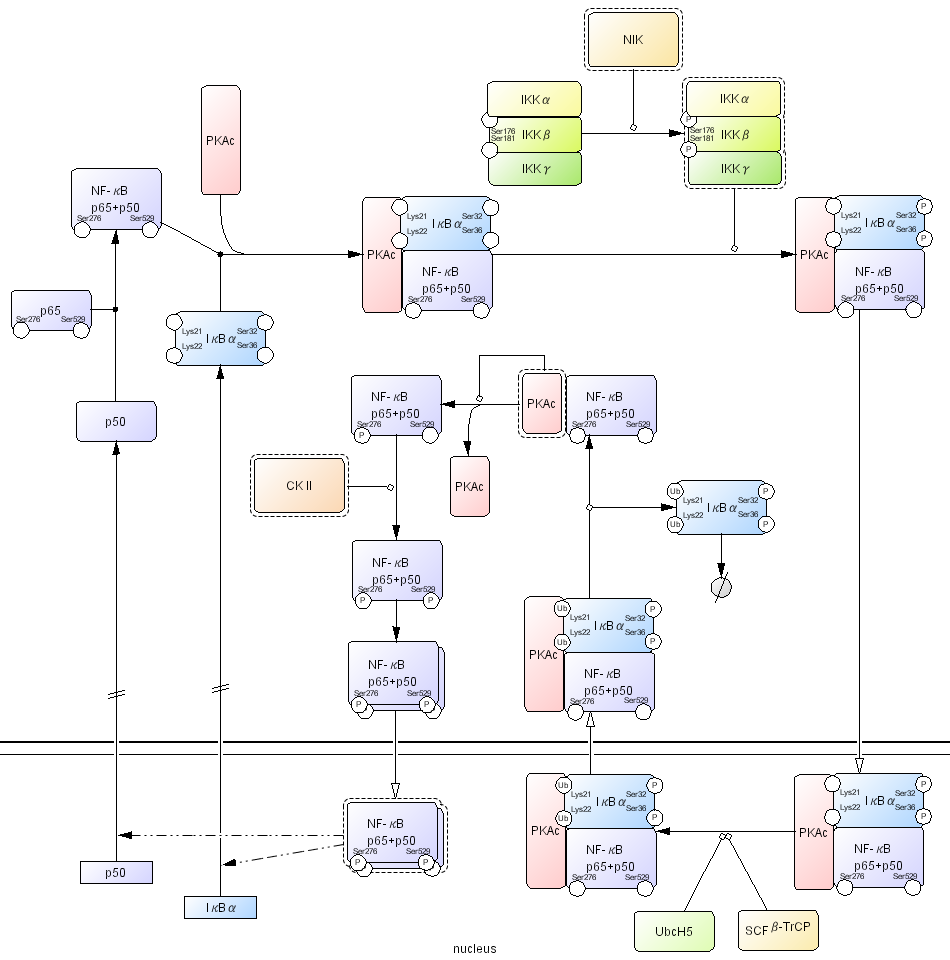
\includegraphics[width=\textwidth]{NF-kB-mechanism/CellDesigner.png}
    \caption{Diagram as created with \celldesigner.}
    \label{fig:process-diagram-old-vs-new:celldesigner}
  \end{subfigure}
  \hspace{1em}
  \begin{subfigure}{0.4\textwidth}
    \centering
    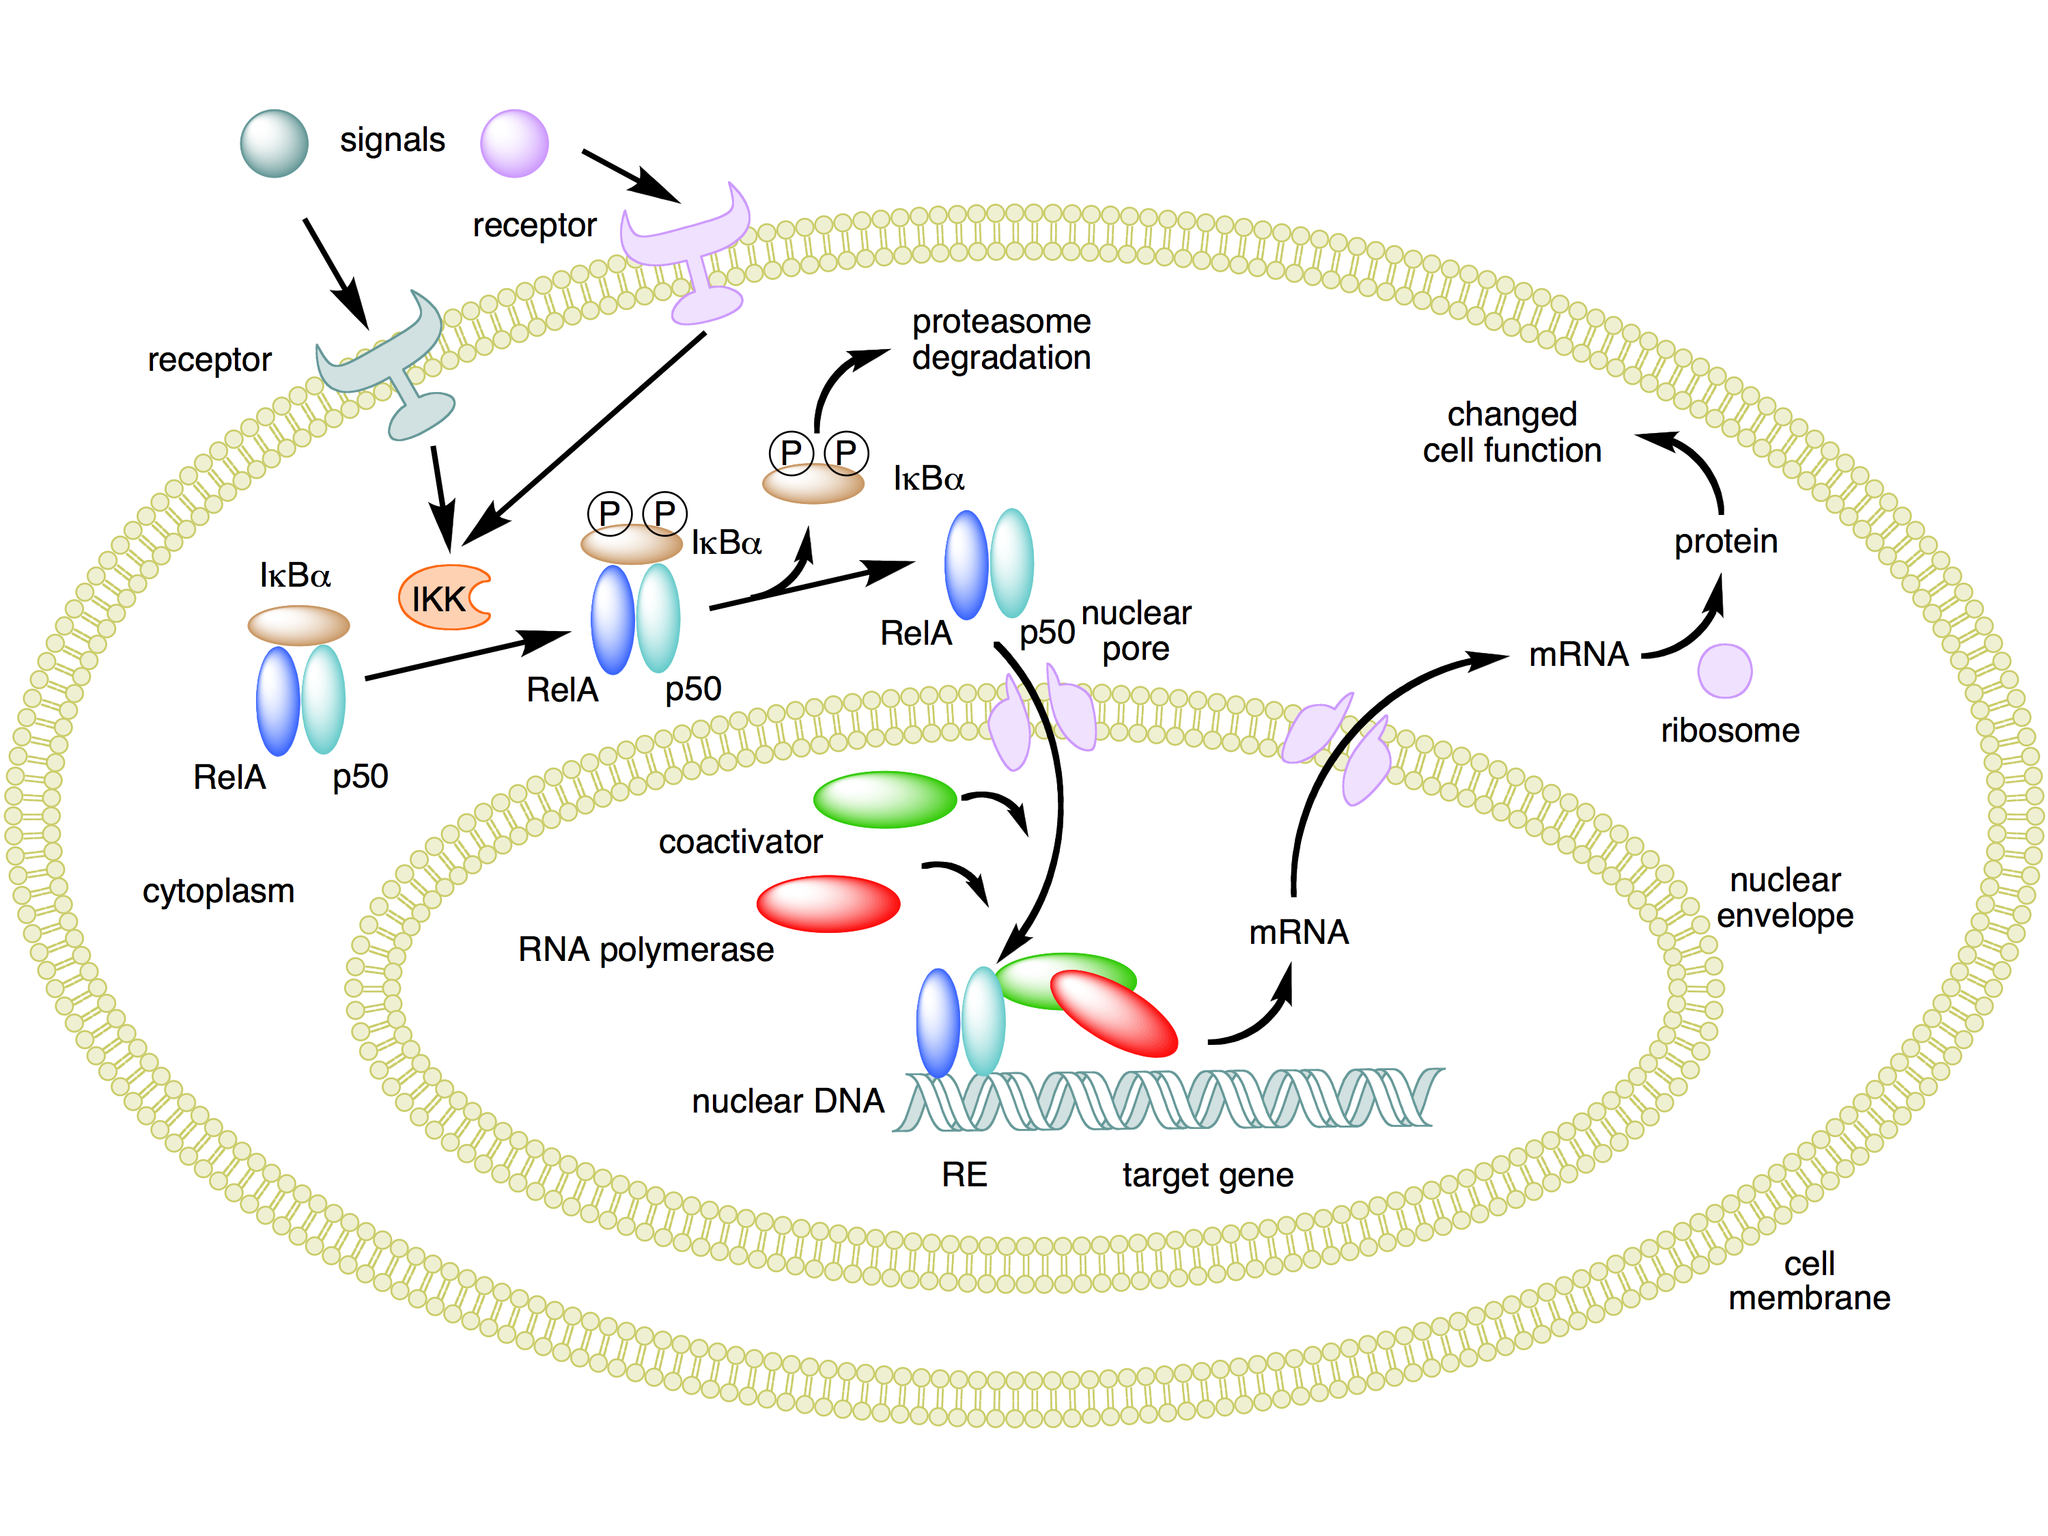
\includegraphics[width=\textwidth]{NF-kB-mechanism/handdrawn.png}
    \caption{Manually created diagram.}
    \label{fig:process-diagram-old-vs-new:handdrawn}
  \end{subfigure}
  \caption{
    Two representations of prototypical mechanisms of \nfkb-signaling.
    % TODO describe roughly what this is for.
    % TODO descibe pros/cons of each
    % TODO describe why this is a nice example for a'' `complex interaction'
  }
  \label{fig:process-diagram-old-vs-new}
\end{figure}
% TODO positioning on page
% TODO replace with image from  http://www.celldesigner.org/features.html ?

% TODO example image of a large disease map

% TODO relationships to other kinds of biological networks


% -------------------------------------
\section{Drawing of Biological Networks / Disease Maps}
\label{sec:draw-biol-netw}
% mainly requirements, and some current research


% -------------------------------------
\section{Ontologies}
\label{sec:ontologies}
% mainly introduce gene ontology

% -------------------------------------
\section{Network Embedding \& Neural Networks}
% only give definitions here
% TODO refer to Related Work for actual research stuff
\label{sec:neural-networks}

\subsection{Embeddings}

\subsection{Neural Networks}

\subsection{Graph Neural Networks}

% TODO define what a SVM is, what supervised learning is...?


% ====================================
\chapter{Related Work}
\label{sec:related-work}
\blindtext

% -------------------------------------
\section{Machine Learning in the Life Sciences}
\label{sec:ml-in-ls}

\subsection{Applications of Graph Neural Networks}
\label{sec:gnn-applications}




% ====================================
\chapter{Methods}
\label{sec:methods}
\blindtext


% -------------------------------------
\section{Datasets \& Preprocessing}
\label{sec:datasets}
\blindtext

\subsection{Datasets used for training and evaluation}


% describe the DMs used, some background, ...., give aliases

% ADReorg (collection)
% ADReorgLast (single)
% PDMap
% ReconMap

% TODO describe inherent differences
\subsection{Graph interpretation}
% how graph is constructed, what considerations one has to make...
Disease maps can be interpreted as bipartite graphs in a natural manner with the
bipartite node sets being the set of reactions and the set of species, respectively.

\subsection{Determining ground-truth Labels}
Although numerous disease maps are publicly available, to the best of our
knowledge none are explicitly annotated with a per-alias label indicating node
duplication. In case we are given a sequence of reorganisation steps $(G_1, ..., G_k)$ % TODO
                                % define reorganisation steps
, we infer node labels by comparing successive steps $G_t$ and $G_{t+1}$. In
case we are given only a single disease map $G$
% TODO calling this G is fishy
, we first construct a collapsed version $G_0$ by collapsing any species aliases
corresponding to the same species into a representative node and moving any edges
incident to aliases to the corresponding representative. We then proceed by
comparing $G_0$ and $G$ like reorganisation steps.
%
In order to make our results comparable to the work of
\citeauthor{nielsen_MachineLearningSupport_2019}, we re-implement the algorithm
employed therein and describe it in detail here for clarity.
%

% TODO (if OK by Sune) describe algorithm

\subsection{Determining Predictors}
% TODO Describe feature sets used, how features are calculated...
% mention that we use igraph?

\section{Classification}
% TODO Describe the methods we use to solve the classification problem
% _not_ the derivations or motivations!

\subsection{Support Vector Machine}

\subsection{Graph Neural Network}


% ====================================
\chapter{Experiments \& Results}
\blindtext


\chapter{Discussion}
\blindtext



\pagebreak

\chapter{First Chapter}

Foo bar baz qux qoo. blblblbl

This is an equation:
\begin{equation}
  \label{eq:foo}
  f(x) = \mat A \mat X
\end{equation}

This is a reference to \refeq{foo}.


\begin{figure}[h]
  \centering
  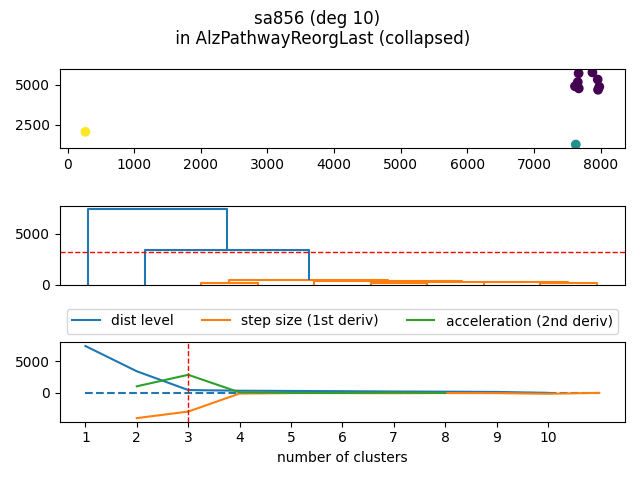
\includegraphics{dummy.png}
  \caption{This is some caption text}
  \label{fig:some-figure}
\end{figure}

This is another reference to \reffig{some-figure}

This is a bib ref \cite{duvenaud_convolutional_2015}.

This is an autor ref: \citeauthor{duvenaud_convolutional_2015} 


\pagelayout{margin} % Restore margins

\chapter{Second Chapter}

\blindtext

\appendix % From here onwards, chapters are numbered with letters, as is the appendix convention

\pagelayout{wide} % No margins
\addpart{Appendix}
\pagelayout{margin} % Restore margins

\chapter{Some more blindtext}

\blindtext

%----------------------------------------------------------------------------------------

\backmatter % Denotes the end of the main document content
\setchapterstyle{plain} % Output plain chapters from this point onwards

%----------------------------------------------------------------------------------------
%	BIBLIOGRAPHY
%----------------------------------------------------------------------------------------

% The bibliography needs to be compiled with biber using your LaTeX editor, or on the command line with 'biber main' from the template directory

\defbibnote{bibnote}{Here are the references in citation order.\par\bigskip} % Prepend this text to the bibliography
\printbibliography[heading=bibintoc, title=Bibliography, prenote=bibnote] % Add the bibliography heading to the ToC, set the title of the bibliography and output the bibliography note

%----------------------------------------------------------------------------------------
%	INDEX
%----------------------------------------------------------------------------------------

% The index needs to be compiled on the command line with 'makeindex main' from the template directory

\printindex % Output the index

\end{document}
